A LaTeX file has a \verb|.tex| extension, and begins with what we call a \emph{preamble} --- declaring the \emph{class} of document, followed by \verb|\begin{document}...\end{document}|.
\lstinputlisting[language=tex,caption={\texttt{example.tex}}]{files/getting-started/example1.tex}

Producing the following output:

\begin{figure}[h]
    \centering
    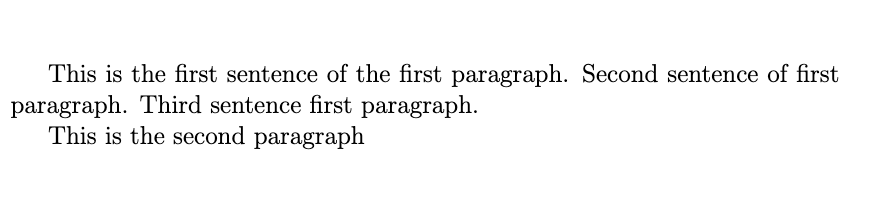
\includegraphics[width=0.8\textwidth]{figures/chapters.png}
    \label{fig:chapters}
\end{figure}

Generally, we declare a document class with \texttt{\textbackslash documentclass[option1, \ldots]\{class\}}, with the most commonly used classes being \verb|article| and \verb|report|.
Every class has a different set of default behaviours, such as \texttt{report} providing a title page.
You can find more options and information on default behaviour on \href{https://texblog.org/2013/02/13/latex-documentclass-options-illustrated/}{this} link.

Default behaviours can also be modified by providing \emph{options}.
You can easily spot them, as they come between square brackets \verb|[]| following some markup.
The option in this example was to change the font size from the default \verb|10pt| to \verb|12pt|.

Another option worth mentioning is \verb|twocolumn|, used to produce two column documents commonly seen in academia.

Later on we will come back to the \emph{preamble} for other important commands.
Generally we create and use templates, so we don't need to remember every small detail, and it becomes quite easy to quickly get your new document up and running.

\subsection{Paragraph}
You will notice that the first paragraph consists of both lines 3 and 4.
This is because a paragraph is only created by having a full empty line (like line 5).
One advantage to separating sentences by a new line is that you can more readily move, copy and delete them in your editor.

Another important feature is that indentation was made automatically.
\LaTeX is smart enough to indent for you and almost always get it right.
If you really want to force a paragraph without indentation, use \verb|\\| at the end of the previous one, like so:
\begin{lstlisting}
    paragraph one\\
    paragraph two not indented.
\end{lstlisting}
% \paragraph{Note} Including an empty line after \verb|\\| will result in a very common warning: \verb|Underfull hbox|. More information on this later in the common errors and warnings section.

\subsection{Sectioning}
Documents with the \texttt{article} class are primarily separated into \verb|section|, \verb|subsection|, \verb|\subsubsection| and \verb|paragraph|, with the first two showing up in a table of contents.
A \texttt{report} has, in addition to the above, \verb|\part| and \verb|\chapter|.

\lstinputlisting[language=tex, caption={\texttt{example2.tex}}]{"./files/getting-started/example2.tex"}

Results in:
\begin{figure}[h]
    \centering
    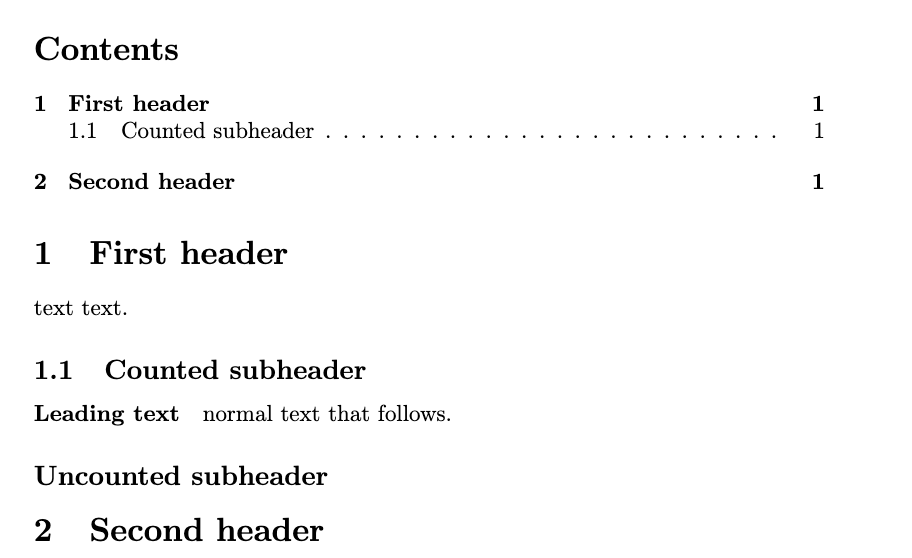
\includegraphics[width=0.6\textwidth]{figures/sections.png}
    \label{fig:sections}
\end{figure}

Every tag that includes some form of counting can have an asterisk (\verb|*|) to remove the counting.
In this case, you can see the difference between \verb|\section{}| and \verb|\section*{}|, and most importantly, the table of contents, generated with \verb|\tableofcontents|, excluded the uncounted subheader.

The \verb|report| class also offers \verb|\chapter(*){}| and \verb|\part(*){}|, relevant mostly to very large documents.

\paragraph{Note:} You will notice that the table of content and the actual content are in the same page. If you want a page break at any point, just use \verb|\pagebreak|!

\subsection{Bold, italic, underline, etc}

\begin{lstlisting}
\textit{Italics}, \underline{underline}, \textbf{bold}.
\textit{Emphasis switches from ``italics'' to \emph{normal}} and \emph{vice-versa} based on context.
\texttt{And we can even get monospace!}
\end{lstlisting}
Results in: \\
\textit{Italics}, \underline{underline}, \textbf{bold}.
\textit{Emphasis switches from ``italics'' to \emph{normal}} and \emph{vice-versa} based on context.
\texttt{And we can even get monospace!}\\

VSCode has a shortcut for these, so you don't need to remember the exact keyword. \verb|Ctrl+L| to initiate a LaTeX command, then \verb|Ctrl+| the first letter of the command --- \verb|Ctrl+i|, \verb|Ctrl+b|, \verb|Ctrl+u|, \verb|Ctrl+e| or \verb|Ctrl+t|, respectively.
So for bold, you would press is \verb|Ctrl+L+Ctrl+B|.
For Mac, just replace \verb|Ctrl| for \verb|Cmd|.

Quotations are done with \textasciigrave\textasciigrave text here \textquotesingle\textquotesingle.
When you type \textasciigrave, the editor will automatically add \textquotesingle.

\paragraph{Note:} Generally the suggestion is to use \verb|\emph{}| over \verb|\textit{}|. Think of it as a ``generic highlighter'' that you can modify with default behaviour to \emph{italicise}, but you could make it change colours or font size or anything else.